\question (西安电子科技大学,1996年)若以1234作为双端队列的输入序列,则既不能由输入受限的双端队列得到,也不能由输出受限的双端队列得到的输出序列是(
)
\par\twoch{1234}{4132}{\textcolor{red}{4231}}{4213}
\begin{solution}输入受限,即一端输入,两端输出。
右入4次得到:1、2、3、4,左出1,左出2,左出3,左出(右出)4,因此得到1234。
右入4次得到:1、2、3、4,右出4,左出1,右出3,右出(左出)2,因此得到4132。
输出受限,即两端输入,一端输出。
左入1,左入2,右入3,左入4,得到4213,四次左出,因此得到4213。
由排除法得到,只有C选项既无法从输入受限的双端队列得到,也无法从输出受限的双端队列得到。
\end{solution}
\question 某队列允许在其两端进行入队操作,但仅允许在一端进行出队操作,若元素a,b,c,d,e依次入此队列后再进行出队操作,则不可能得到的出队序列是(
)
\par\twoch{b,a,c,d,e}{d,b,a,c,e}{\textcolor{red}{d,b,c,a,e}}{e,c,b,a,d}
\begin{solution}仅允许在一端进行出队操作,为了方便,假设在左端进行出队操作。则队列顺序即为出队序列。
根据入队顺序和出队顺序求入队操作的情况。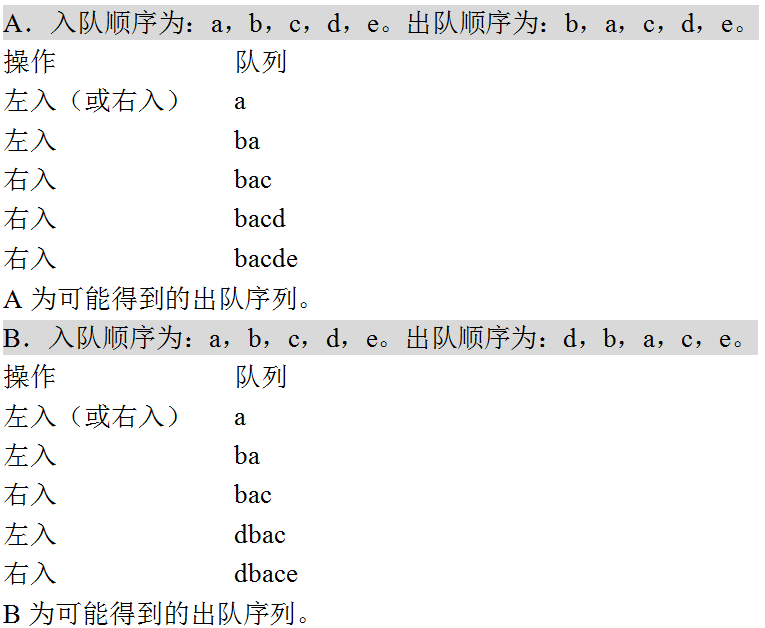
\includegraphics[width=3.46875in,height=2.84375in]{computerassets/E077C7E626914B317B104E76339250DD.png}
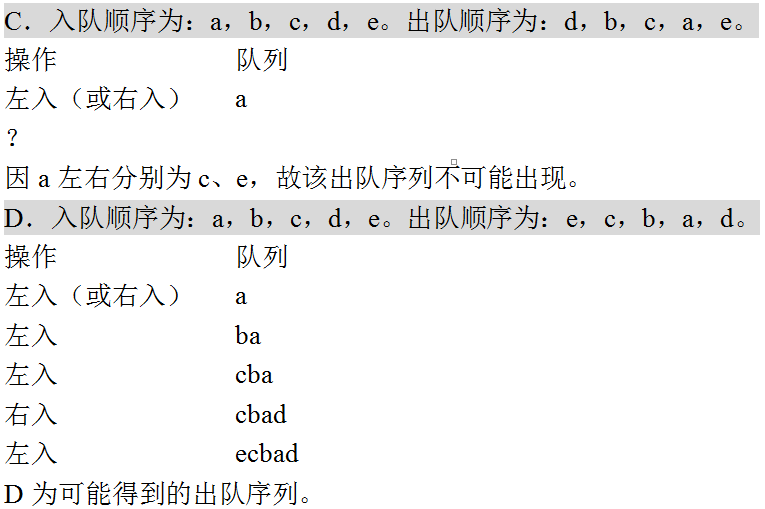
\includegraphics[width=3.46875in,height=2.31250in]{computerassets/B94FE2E65B14D5127E7618D80587CA88.png}
【总结】快速解题,无论哪种入队方式(即先从左边入队还是先从右边入队),a和b都应该相邻,这是出队序列合理的必要条件。只有选项C所给序列中a与b不相邻。故C为不可能出现的出队序列。
\end{solution}
\question 设有一个n阶三对角线矩阵A{[}n{]}{[}n{]},现把它的三条对角线上的非零元素按行存放到一个一维数组B{[}{]}中,A{[}1{]}{[}1{]}存放到B{[}1{]}中(假定不用0下标),那么B{[}k{]}存放的元素的行号是(
)
\par\twoch{(k+1)/3向下取整}{\textcolor{red}{(k+1)/3向上取整}}{(k+2)/3向下取整}{(k+2)/3向上取整}
\begin{solution}这种题目最好采用特殊值法,推导过程可能比较繁琐,见表
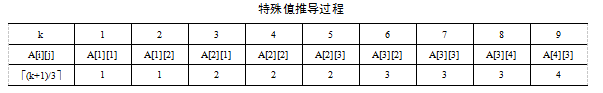
\includegraphics[width=6.28125in,height=0.96875in]{computerassets/ecd0148ec7917beabeba93b448a52f92.png}
\end{solution}
\question 若将n阶上三角矩阵A按照列优先顺序存放在一维数组B{[}0,1,,\{n×(n+1)/2\}-1{]}中,第一个非零元素a(1,1)存于B{[}0{]}中,则存放到B{[}k{]}中的非零元素a(i,j)(1≤i≤n,1≤j≤n)的下标i、j与k的对应关系是(
)
\par\twoch{k=i×(i+1)/2+j}{k=i×(i-1)/2+j-1}{k=j×(j+1)/2+i}{\textcolor{red}{k=j×(j-1)/2+i-1}}
\begin{solution}对于元素a(i,j)而言,前面有j-1列,第1列到第j-1列的元素个数分别为1~j-1个,由等差数列求和公式可算得一共有j×(j-1)/2个元素,故k=j×(j-1)/2+i-1(注意B数组是从0开始存元素,因此要减去1)
\end{solution}
\question (华中科技大学,2005年)一个n*n的对称矩阵,如果以行或列为主序放入内存,则容量为(
)
\par\twoch{\textcolor{red}{n(n+1)/2}}{n*n/2}{(n+1)*(n+1)/2}{n*n}
\begin{solution}一个n*n的对称矩阵,如果以行或列为主序放入内存,则容量为:(1+2+3+\ldots{}+n)=n(n+1)/2
\end{solution}
\question (华南理工大学,2006年)稀疏矩阵的三元组存储方法( )
\par\fourch{实现转置运算很简单,只需将每个三元组中的行标和列表交换}{是一种链式存储方法}{\textcolor{red}{矩阵的非零元个数和位置在操作过程中变化不大时较有效}}{比十字链表法更高效}
\begin{solution}A稀疏矩阵还要实现三元组之间的重新排列,所以A错误。B不是链式存储,利用数组存储,D与十字链表相比需要根据使用情况的不同来定。
\end{solution}
\question (中山大学,2005年)用十字链表表示一个稀疏矩阵,每个非零元一般用一个含有(
)个域的节点表示
\par\twoch{2}{3}{4}{\textcolor{red}{5}}
\begin{solution}存储稀疏矩阵的十字链表节点包含5个域:该非零元的行下表、该非零元的列下表、该非零元的值、该非零元所在行表的后继链域,以及该非零元所在列表的后继链域
\end{solution}
\question (重庆大学,2005年)在稀疏矩阵A(n*n)的十字链表表示中,表头节点的个数为(
)
\par\twoch{n}{n+1}{\textcolor{red}{2n}}{2n+1}
\begin{solution}在用十字链表存储稀疏矩阵时,有n个表头结点指向n个行,下面指向的是存储每一行非零元素的一个链表,同样的有n个表头结点指向n个列,一共有2n个表头
\end{solution}
